\documentclass[tikz]{standalone}
\usepackage[utf8]{inputenc}
\usepackage{amsmath}

\usetikzlibrary{calc}

\def\hash{\mathrm{H}}

\begin{document}

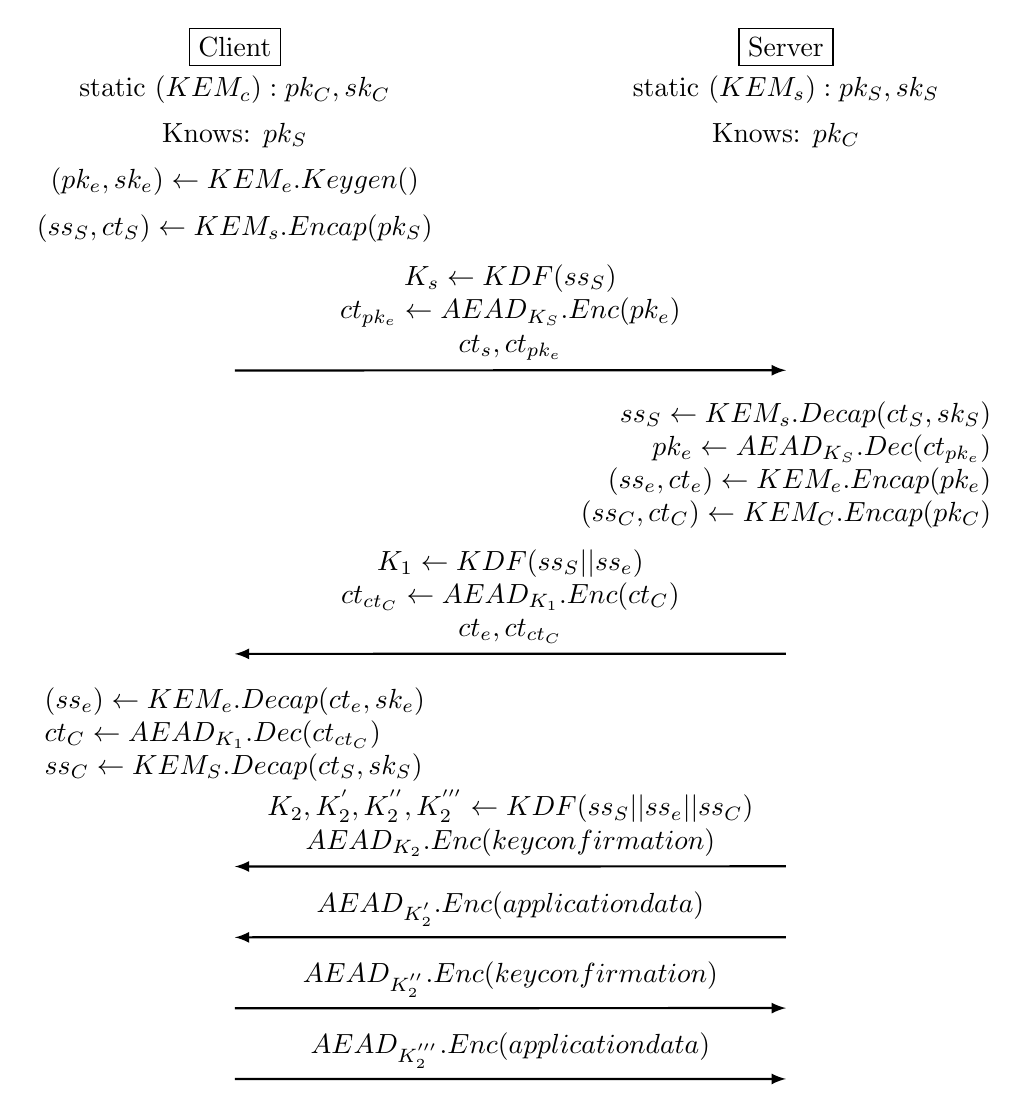
\begin{tikzpicture}[yscale=.9,xscale=.7]
\tikzstyle{box}=[draw,fill=white, rectangle, rounded corners=3pt, align=left, minimum width=5.7cm, minimum height=.8cm]
  
% Public parameters and password

  
% Alice: generate public data

\node[draw] (Alice) at (-5,0) {Client}; 
%\draw[thick] (Alice) -- ++(0, -12.5);
\node[below, align=left] (Long-term key Alice) at (Alice.south) {static ($KEM_c): pk_C,sk_C$};
%\usepackage{fixltx2e} 
%like\textsubscript{this}
%were made by \emph{accident}.
\node[below, align=left](kA) at (Long-term key Alice.south) { Knows: $pk_S$};
%\node[box] (initalice) at ($(Alice) + (0,-2.5)$) {random $a$ in $[1, q-1]$ \\ $A \gets g^a$};
\node[below, align=left] (initalicekg) at (kA.south) {($pk_e,sk_e) \gets KEM_e.Keygen()$};
\node[below, align=left] (initaliceencap) at (initalicekg.south) {($ss_S,ct_S) \gets KEM_s.Encap(pk_S)$};

%$ x_{12345} \quad x_12
% Bob: generate public data
\node[draw] (Bob) at (5,0) {Server};
%\draw[thick] (Bob) -- ++ (0, -12.5);
\node[below] (Long-term key Bob) at (Bob.south) {static ($KEM_s): pk_S,sk_S$};
\node[below, align=right](kB) at (Long-term key Bob.south) { Knows: $pk_C$};
%\node[below right , align=left] at (Bob.south) {secret: $v:= g^x$ \\ other: salt};

\draw[-latex,thick,align=center] ($(kA.south) + (0, -3)$) -- ($(kB.south) + (0, -3)$) node [pos=0.5, above](handshake1) {$K_s \gets KDF(ss_S)$\\ $ct_{pk_e}\gets AEAD_{K_S}.Enc(pk_e)$ \\
$ct_s,ct_{pk_e}$};

% Alice and Bob: generate secret key
\node[below, align=right] (processbob) at ($(kB.south) + (0,-3.3)$) {$ss_S \gets KEM_s.Decap(ct_S,sk_S)$\\  $pk_e\gets AEAD_{K_S}.Dec(ct_{pk_e})$\\ ($ss_e,ct_e) \gets KEM_e.Encap(pk_e)$ \\$(ss_C,ct_C)\gets  KEM_C.Encap(pk_C)$};

\draw[-latex,thick,align=center] ($(kB.south) + (0, -7)$) -- ($(kA.south) + (0, -7)$) node [pos=0.5, above](handshake2) {$K_1\gets KDF(ss_S||ss_e)$\\$ct_{ct_C}\gets AEAD_{K_1}.Enc(ct_C)$\\$ct_e,ct_{ct_C}$};
\node[below, align=left] (processalice) at ($(initaliceencap.south)+ (0,-6)$){($ss_e) \gets KEM_e.Decap(ct_e,sk_e)$\\$ct_C\gets AEAD_{K_1}.Dec(ct_{ct_C})$\\$ss_C\gets KEM_S.Decap(ct_S,sk_S)$};

\draw[-latex,thick,align=center] ($(kB.south) + (0, -10)$) -- ($(kA.south) + (0, -10)$) node [pos=0.5, above]{$K_2,K_2^{'},K_2^{''},K_2^{'''}\gets KDF(ss_S||ss_e||ss_C)$\\$AEAD_{K_2}.Enc(key confirmation)$};
\draw[-latex,thick,align=center] ($(kB.south) + (0, -11)$) -- ($(kA.south) + (0, -11)$) node [pos=0.5, above]{$AEAD_{K_2^{'}}.Enc(application data)$};
\draw[-latex,thick,align=center] ($(kA.south) + (0, -12)$) -- ($(kB.south) + (0, -12)$) node [pos=0.5, above]{$AEAD_{K_2^{''}}.Enc(key confirmation)$};
\draw[-latex,thick,align=center] ($(kA.south) + (0, -13)$) -- ($(kB.south) + (0, -13)$) node [pos=0.5, above]{$AEAD_{K_2^{'''}}.Enc(application data)$};
%\node[box,below] (processbob) at ($(kB.south) + (0, -2)$) {$u \gets \hash(A, B)$ \\ $s_k \gets \hash((Av^u)^b)$};
 
% verification if the session key is the same
%\node[box,below] (verifbob) at ($(processalice.south) + (10,-1)$) {Verify $M_1$\\ $M_2 \gets \hash(A, M_1, s_k)$};
%\node[box,below] (verifalice) at ($(verifbob.south) + (-10,-1)$) {Verify $M_2$};

% labels on arrows

%\draw[-latex,thick] ($(kB.south) + (0, -1)$) -- ($(initalicekg.south) + (0, -1.5)$) node [pos=0.5, above] {$B$, salt};

%\draw[-latex,thick] ($(processalice.south) + (0, -.5)$) --++ (10, 0) node [pos=0.5, above] {$M_1$};
%\draw[-latex,thick] ($(verifbob.south) + (0, -.5)$) --++ (-10,0) node [pos=0.5, above] {$M_2$};

\end{tikzpicture}

\end{document}